\documentclass[twoside,10pt]{report}
\usepackage{toggles}
%\toggletrue{sectionbreaks}
\newcommand{\docTitle}{Holomorphic Dynamics}
\usepackage{common}
\importStyles{formal}{rainbow}{lined}

%\renewcommand{\theenumi}{\alph{enumi}}

\begin{document}
\toc
%\header{text}{text}
\footer

%+-------------------+
%| +---------------+ |
%| |    Chapter    | |
%| +---------------+ |
%+-------------------+
% Polynomial dynamics

\chapter{Polynomial dynamics}

%--------------------------------------------------------------------------------
% Introduction
%--------------------------------------------------------------------------------
\section{Introduction}

Take some polynomial $p: \mathbb{C}\to \mathbb{C}$, then we can consider the orbits $\left\{ p^{n}(z) \right\}_{n=1}^{\infty}$ for any $z \in \mathbb{C}$, where $p^{n}$ denotes repeatedly applying $p$ a total of $n$ times.

\begin{defn}[]
Given a polynomial $p:\mathbb{C}\to \mathbb{C}$,
\begin{itemize}
	\item $I_{p} := \left\{ z \in \mathbb{C} \;|\; \lim_{n \to \infty} p^{n}(z) \right\}$ is the \textbf{set of escaping points} of $p$;
	\item $K_{p} := \mathbb{C} - I_{p}$ is the \textbf{filled Julia set} of $p$;
	\item $J_{p} := \p K_{p}$ is the \textbf{Julia set} of $p$.
\end{itemize}
\end{defn}
$I_{p}$ is nonempty if $\deg(p) \geq 2$. This is because as $|z|$ gets large enough, $|p^{n}(z)| \approx |z|^{(k^{n})}$, which clearly diverges as $n\to \infty$.

One way of thinking of $I_{p}$ is as the set of points converging to the point at infinity inside the Riemann sphere $\mathbb{\hat{C}}$. This is helpful because, as we'll see later on, the Julia set contains the ``chaotic" points that neither converge nor get stuck in a cycle during the process of iterating $p$. The rest of the points in the plane (so $I_{p}$ and the interior of $K_{p}$) either converge (perhaps to the point at infinity) or get stuck in a cycle.

\begin{ex}[]
Let $p(z) = z^2$, then
\begin{itemize}
	\item $I_{p} = \left\{ z\in \mathbb{C}\;|\; |z| > 1 \right\}$;
	\item $K_{p} = \left\{ z\in\mathbb{C} \;|\; |z|\leq 1 \right\}$;
	\item $J_{p} = \left\{ z\in\mathbb{C} \;|\; |z|=1 \right\}$.
\end{itemize}
\end{ex}

For many simple polynomials, the Julia set is a fractal. The below is a first attempt at giving this a concrete definition, although we'll move to better definitions later on.

\begin{defn}[]
A closed set $E \subseteq \mathbb{C}$ is a \textbf{fractal set} if it's \textit{not} a countable union of rectifiable (finite length) curves. A domain (nonempty, connected, open set) $D$ in $\mathbb{C}$ is a \textbf{fractal domain} if $\p D$ is a fractal set.
\end{defn}

\warn{Fill in gap here...}

\begin{thrm}[]
Let $\deg(p) \geq 2$, then
\begin{enumerate}
	\item $K_{p}$ is a nonempty compact set;
	\item $I_{p}$ is a domain (nonempty, connected, open).
\end{enumerate}
\end{thrm}
\begin{figure}[H]
	\centering
	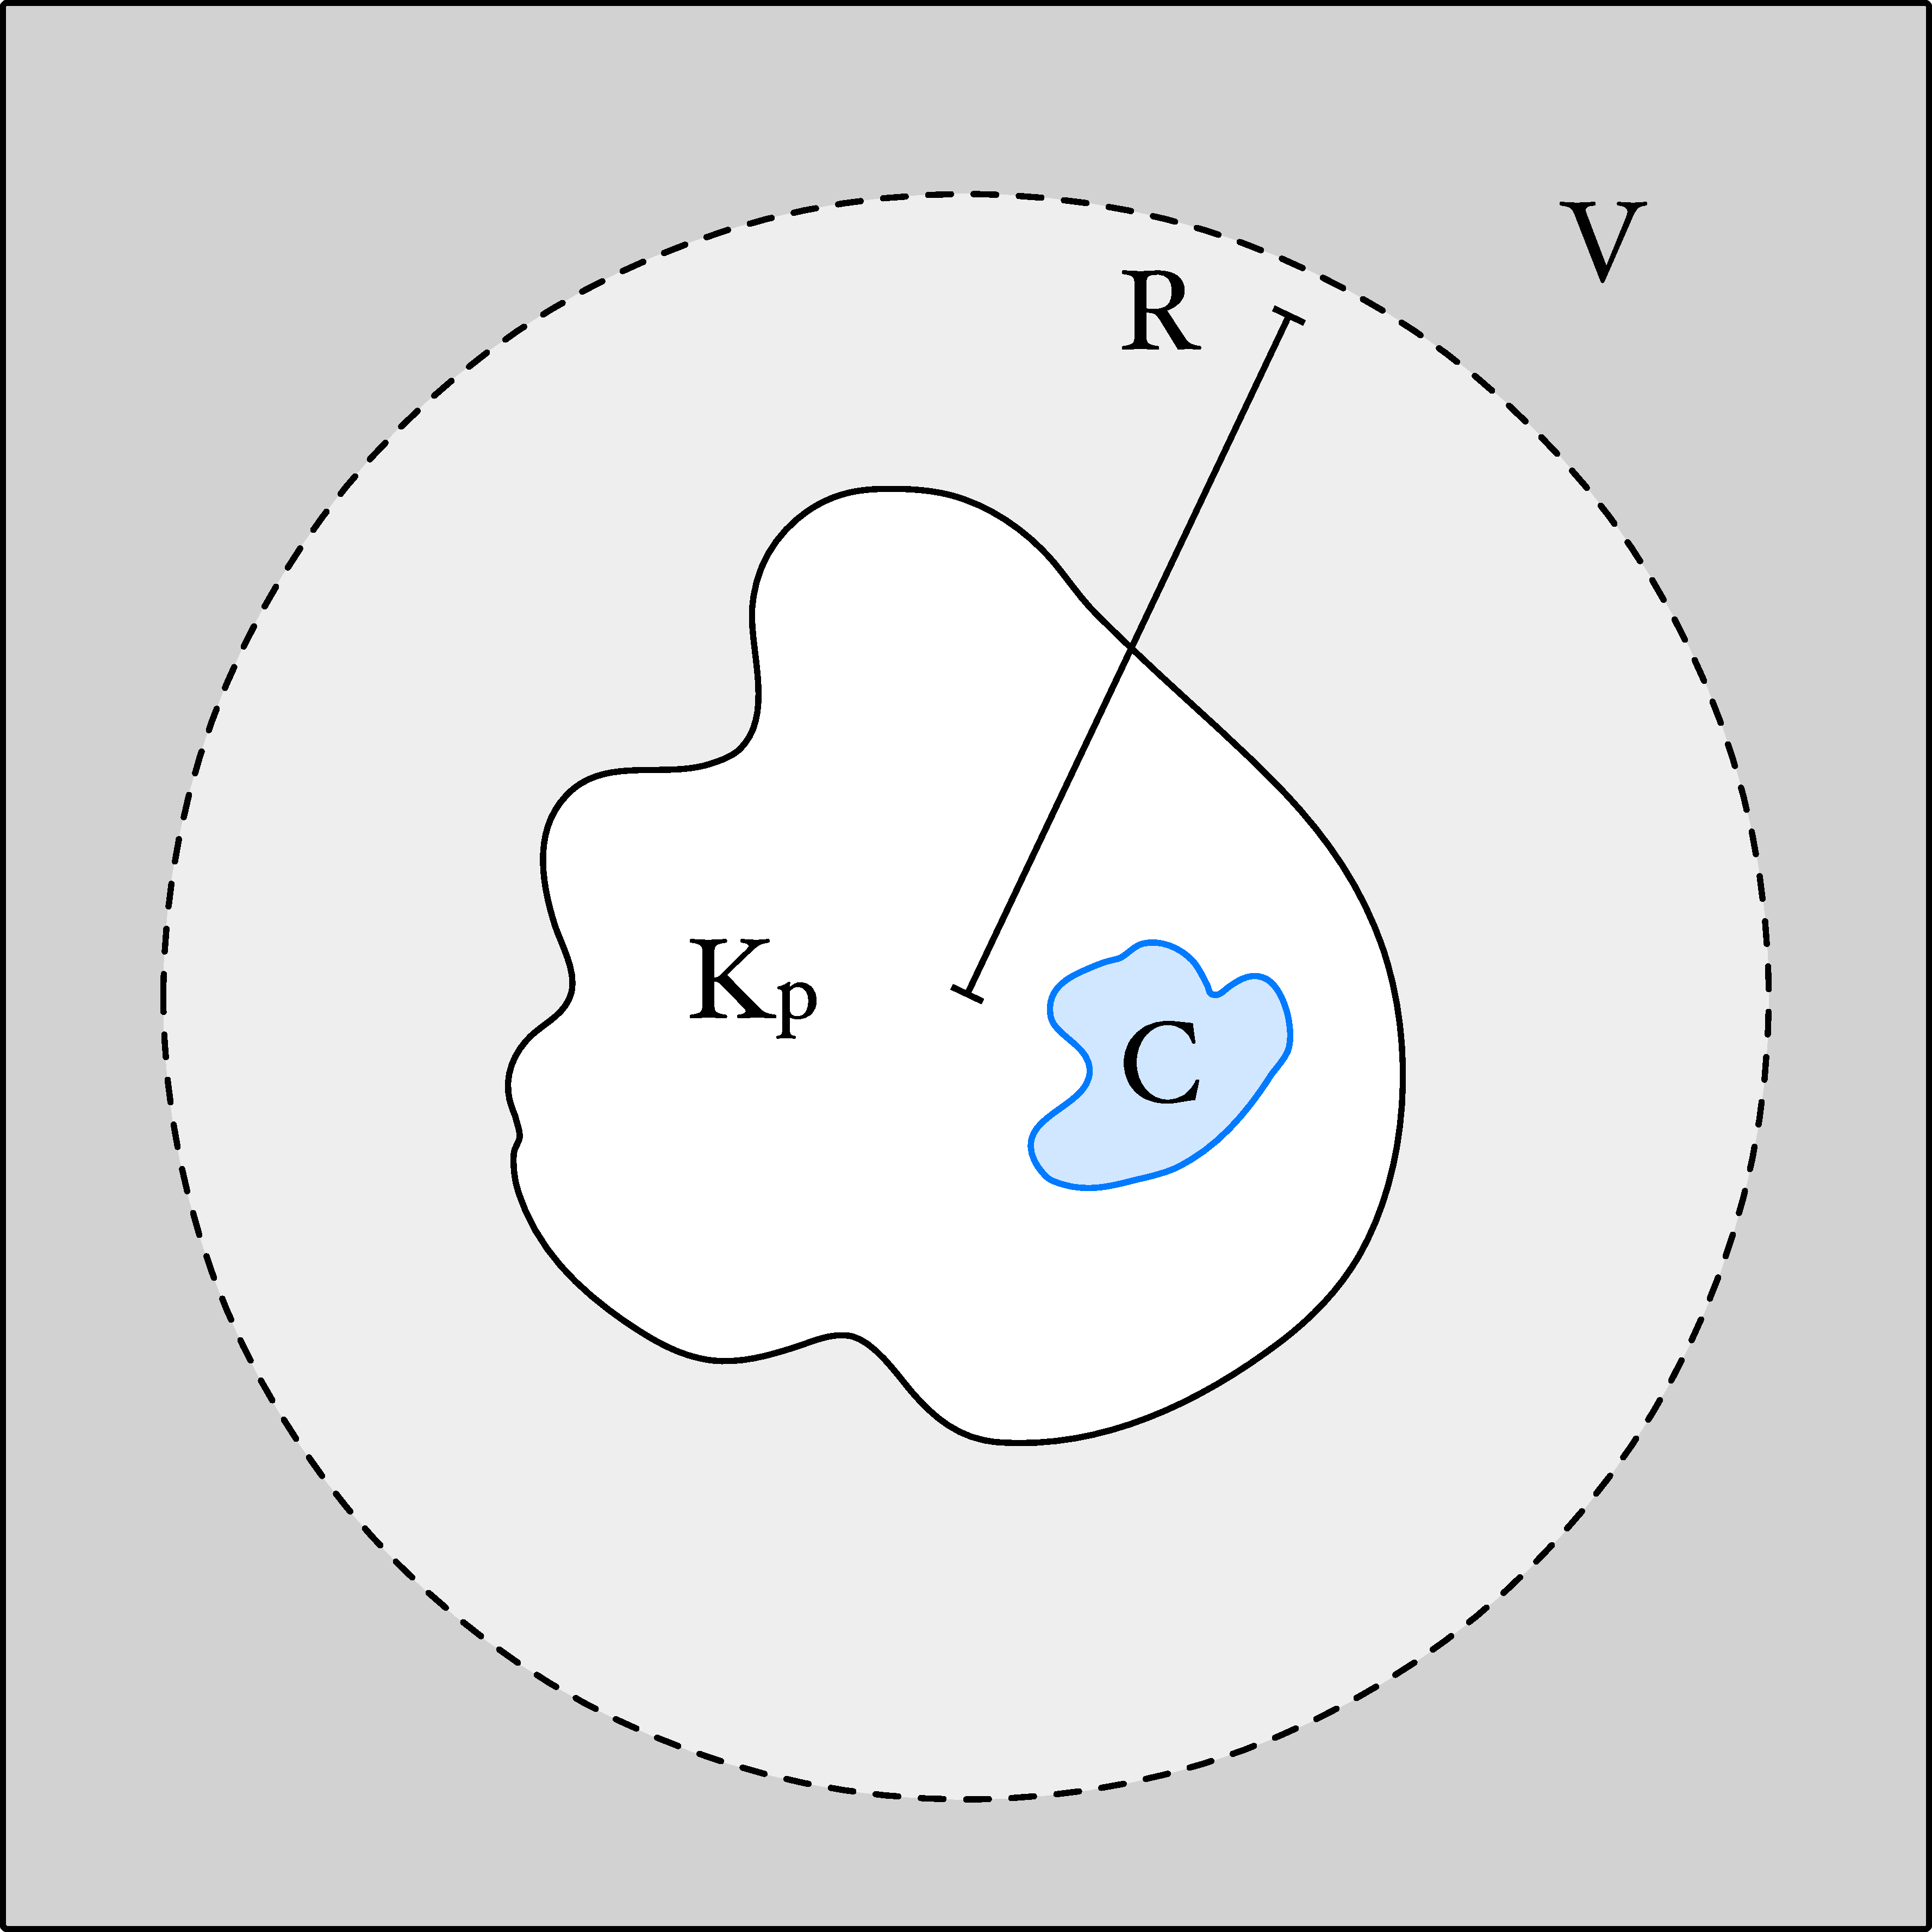
\includegraphics[scale=.1]{fig/julia_connected.pdf}
	%\caption{}
\end{figure}


\end{document}
